\documentclass[12pt,a4paper]{article}

% ============================================================================
% PACKAGES
% ============================================================================
\usepackage[utf8]{inputenc}
\usepackage[T1]{fontenc}
\usepackage{lmodern}
\usepackage[english]{babel}
\usepackage{amsmath,amssymb}
\usepackage{graphicx}
\usepackage{xcolor}
\usepackage{hyperref}
\usepackage{listings}
\usepackage{booktabs}
\usepackage{longtable}
\usepackage{multirow}
\usepackage{caption}
\usepackage{geometry}
\usepackage{fancyhdr}
\usepackage{setspace}
\usepackage{tikz}
\usepackage{float}
\usepackage{enumitem}

% ============================================================================
% CONFIGURATION
% ============================================================================
\geometry{margin=1in}
\usetikzlibrary{shapes,arrows.meta,positioning,calc,fit,backgrounds,decorations.pathreplacing}

\hypersetup{
    colorlinks=true,
    linkcolor=blue!60!black,
    citecolor=green!50!black,
    urlcolor=blue!70!black
}

% Code listing configuration
\definecolor{codebg}{rgb}{0.95,0.95,0.95}
\definecolor{codegreen}{rgb}{0,0.6,0}
\definecolor{codegray}{rgb}{0.5,0.5,0.5}
\definecolor{codepurple}{rgb}{0.58,0,0.82}
\definecolor{ctxcyan}{HTML}{06B6D4}
\definecolor{ctxdark}{HTML}{0F172A}

\lstdefinestyle{code}{
    backgroundcolor=\color{codebg},
    commentstyle=\color{codegreen},
    keywordstyle=\color{blue},
    numberstyle=\tiny\color{codegray},
    stringstyle=\color{codepurple},
    basicstyle=\ttfamily\footnotesize,
    breakatwhitespace=false,
    breaklines=true,
    captionpos=b,
    keepspaces=true,
    numbers=left,
    numbersep=5pt,
    showspaces=false,
    showstringspaces=false,
    showtabs=false,
    tabsize=2,
    language=Java,
    morekeywords={async,await,interface,type,export,import,const,let,from}
}

\lstdefinestyle{terminal}{
    backgroundcolor=\color{ctxdark},
    basicstyle=\ttfamily\footnotesize\color{white},
    breaklines=true,
    frame=single,
    rulecolor=\color{ctxdark},
    numbers=none
}

\lstset{style=code}

% Page style
\pagestyle{fancy}
\fancyhf{}
\fancyhead[L]{\leftmark}
\fancyhead[R]{\thepage}
\renewcommand{\headrulewidth}{0.4pt}

% Spacing
\onehalfspacing

% ============================================================================
% TITLE
% ============================================================================
\title{\textbf{ctx-sys: Intelligent Context Management\\for AI-Assisted Software Development}\\[0.5cm]
{\large Local Hybrid RAG with Graph Traversal, Semantic Search, and Conversation Memory}}

\author{David Franz}
\date{February 2026}

% ============================================================================
% DOCUMENT BEGIN
% ============================================================================
\begin{document}

\maketitle

% ============================================================================
% ABSTRACT
% ============================================================================
\begin{abstract}
Modern AI coding assistants face a fundamental limitation: context windows are too small to hold an entire codebase, its documentation, and the history of decisions made about it. This paper presents \textbf{ctx-sys}, an open-source context management system that solves this through a local-first hybrid RAG architecture.

ctx-sys indexes codebases using tree-sitter AST parsing, generates semantic embeddings with Ollama, and builds a relationship graph connecting functions, classes, imports, and documentation. At query time, three retrieval strategies---vector similarity, full-text search with BM25, and graph traversal---are combined via Reciprocal Rank Fusion (RRF) to find precisely the right context.

The system runs entirely locally with no cloud dependencies, stores everything in a single SQLite database, and integrates with AI assistants through the Model Context Protocol (MCP). Advanced features include HyDE query expansion, multi-vector chunking for large entities, conversation memory with decision tracking, and agent-oriented memory management.

The implementation comprises approximately 20,000 lines of TypeScript with 1,668 tests across 65 test suites. It supports TypeScript, Python, Rust, Go, Java, C/C++, and C\#, with document indexing for Markdown, HTML, PDF, CSV, XML, and other structured formats.

\medskip
\noindent\textbf{Keywords:} Retrieval-Augmented Generation, Context Management, AI Coding Assistants, Graph RAG, Local-First, MCP
\end{abstract}

\tableofcontents
\newpage

% ============================================================================
% SECTION 1: INTRODUCTION
% ============================================================================
\section{Introduction}
\label{sec:introduction}

\subsection{The Context Problem}

AI coding assistants built on Large Language Models have transformed software development. Tools like Claude, GitHub Copilot, and Cursor demonstrate remarkable capabilities in code generation, explanation, and debugging. However, they share a fundamental limitation: \textit{context constraints}.

Even with context windows reaching 200,000 tokens, they remain insufficient for comprehensive development tasks:

\begin{itemize}
    \item \textbf{Codebase scale}: A 100,000-line project exceeds any practical context window
    \item \textbf{Information dispersion}: Relevant context is scattered across source files, documentation, commit history, and past conversations
    \item \textbf{Conversation drift}: Extended sessions accumulate decisions and understanding that degrades as conversations exceed limits
    \item \textbf{Dependency complexity}: Understanding one function may require tracing imports, types, and base classes across dozens of files
\end{itemize}

Simply expanding context windows is not the answer. Token costs scale linearly, attention mechanisms are quadratic, and larger contexts do not solve the problem of \textit{relevance}---determining which information among vast repositories actually pertains to the current task.

\subsection{The Smart Librarian Paradigm}

ctx-sys adopts a ``smart librarian'' approach: rather than hoarding everything into context, it knows \textit{where} information exists and retrieves only what matters. This manifests as:

\begin{enumerate}
    \item \textbf{Index} the codebase, documentation, and conversation history
    \item \textbf{Extract} entities, relationships, and semantic meaning
    \item \textbf{Retrieve} precisely the right context on demand
    \item \textbf{Assemble} context with source attribution, respecting token budgets
\end{enumerate}

The result: AI assistants that have access to everything but only surface what's relevant.

\subsection{Contributions}

This paper makes the following contributions:

\begin{enumerate}
    \item A \textbf{hybrid retrieval architecture} combining vector similarity, graph traversal, and full-text search with Reciprocal Rank Fusion
    \item \textbf{Code-aware indexing} using tree-sitter AST parsing with automatic relationship extraction across 7 programming languages
    \item \textbf{Advanced retrieval techniques} including HyDE query expansion, multi-vector chunking, retrieval gating, and smart context expansion
    \item \textbf{Conversation memory} with decision extraction and session management for persistent knowledge
    \item A complete \textbf{reference implementation} with MCP integration, 12 action-based tools, and production-ready deployment as an npm package
\end{enumerate}


% ============================================================================
% SECTION 2: SYSTEM ARCHITECTURE
% ============================================================================
\section{System Architecture}
\label{sec:architecture}

\subsection{Architecture Overview}

Figure~\ref{fig:architecture} shows the overall system architecture. ctx-sys sits between developer tools and AI assistants, providing intelligent context retrieval through the Model Context Protocol.

\begin{figure}[H]
\centering
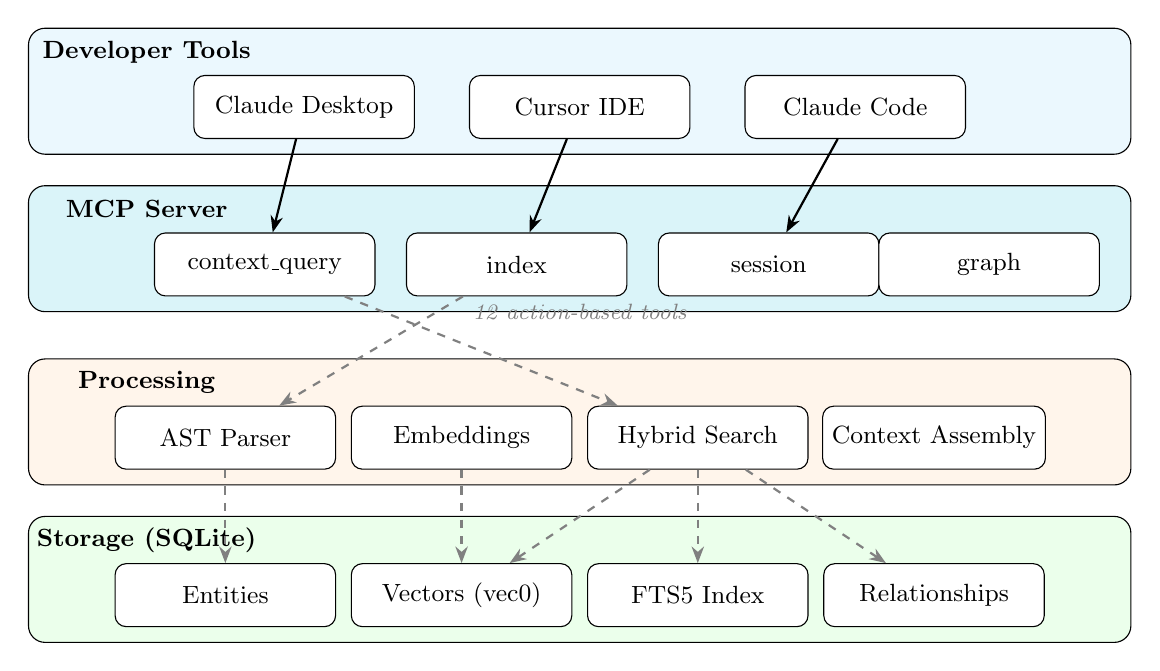
\begin{tikzpicture}[
    node distance=0.8cm,
    box/.style={rectangle, draw, rounded corners=4pt, minimum width=2.8cm, minimum height=0.8cm, font=\small},
    layer/.style={rectangle, draw, rounded corners=6pt, fill=#1, minimum width=14cm, minimum height=1.6cm, font=\small\bfseries},
    arrow/.style={-{Stealth[length=6pt]}, thick},
    label/.style={font=\footnotesize\itshape, text=gray}
]

% Integration layer
\node[layer=cyan!8] (integration) at (0,6) {};
\node[font=\small\bfseries] at (-5.5,6.5) {Developer Tools};
\node[box, fill=white] (claude) at (-3.5,5.8) {Claude Desktop};
\node[box, fill=white] (cursor) at (0,5.8) {Cursor IDE};
\node[box, fill=white] (code) at (3.5,5.8) {Claude Code};

% MCP layer
\node[layer=ctxcyan!15] (mcp) at (0,4) {};
\node[font=\small\bfseries] at (-5.5,4.5) {MCP Server};
\node[box, fill=white] (search) at (-4,3.8) {context\_query};
\node[box, fill=white] (index) at (-0.8,3.8) {index};
\node[box, fill=white] (memory) at (2.4,3.8) {session};
\node[box, fill=white] (graph) at (5.2,3.8) {graph};
\node[label] at (0,3.2) {12 action-based tools};

% Processing layer
\node[layer=orange!8] (processing) at (0,1.8) {};
\node[font=\small\bfseries] at (-5.5,2.3) {Processing};
\node[box, fill=white] (ast) at (-4.5,1.6) {AST Parser};
\node[box, fill=white] (embed) at (-1.5,1.6) {Embeddings};
\node[box, fill=white] (retrieval) at (1.5,1.6) {Hybrid Search};
\node[box, fill=white] (context) at (4.5,1.6) {Context Assembly};

% Storage layer
\node[layer=green!8] (storage) at (0,-0.2) {};
\node[font=\small\bfseries] at (-5.5,0.3) {Storage (SQLite)};
\node[box, fill=white] (entities) at (-4.5,-0.4) {Entities};
\node[box, fill=white] (vectors) at (-1.5,-0.4) {Vectors (vec0)};
\node[box, fill=white] (fts) at (1.5,-0.4) {FTS5 Index};
\node[box, fill=white] (rel) at (4.5,-0.4) {Relationships};

% Arrows
\draw[arrow] (claude) -- (search);
\draw[arrow] (cursor) -- (index);
\draw[arrow] (code) -- (memory);
\draw[arrow, dashed, gray] (search) -- (retrieval);
\draw[arrow, dashed, gray] (index) -- (ast);
\draw[arrow, dashed, gray] (retrieval) -- (vectors);
\draw[arrow, dashed, gray] (retrieval) -- (fts);
\draw[arrow, dashed, gray] (retrieval) -- (rel);
\draw[arrow, dashed, gray] (ast) -- (entities);
\draw[arrow, dashed, gray] (embed) -- (vectors);

\end{tikzpicture}
\caption{ctx-sys system architecture. Developer tools connect via MCP. The processing layer handles indexing and retrieval. All data lives in a single SQLite database.}
\label{fig:architecture}
\end{figure}

\subsection{Design Principles}

The architecture is guided by four principles:

\begin{description}
    \item[Local-first] All processing happens on the developer's machine. Ollama provides local embeddings and summarization. The database is a single SQLite file. No API keys required for core functionality.

    \item[Incremental] Only changed files are re-indexed. Content hashing detects modifications. Embedding generation is hash-gated so unchanged entities skip expensive LLM calls.

    \item[Multi-strategy retrieval] No single search strategy works for all queries. Keyword search excels at exact identifiers. Semantic search handles conceptual queries. Graph traversal discovers structural relationships. Combining all three through RRF produces consistently better results than any single approach.

    \item[MCP-native] The primary interface is the Model Context Protocol---an open standard for connecting AI assistants to external data sources. This makes ctx-sys compatible with any MCP client without custom integration code.
\end{description}

\subsection{Storage Layer}

Everything lives in a single SQLite database enhanced with two extensions:

\begin{itemize}
    \item \textbf{FTS5} --- SQLite's built-in full-text search with BM25 ranking for keyword queries
    \item \textbf{sqlite-vec} --- native vector search extension providing \texttt{vec0} virtual tables for cosine similarity KNN queries
\end{itemize}

The database stores entities (code symbols, document sections), their vector embeddings, a relationship graph, conversation history, and agent state---all in a portable, single-file format.


% ============================================================================
% SECTION 3: CODE INTELLIGENCE
% ============================================================================
\section{Code Intelligence}
\label{sec:code-intelligence}

\subsection{Multi-Language AST Parsing}

ctx-sys parses source code into Abstract Syntax Trees, extracting meaningful entities from seven programming languages, all using tree-sitter WASM grammars for precise, cross-platform parsing:

\begin{table}[H]
    \centering
    \caption{Supported languages and extracted entities}
    \label{tab:languages}
    \begin{tabular}{llp{8cm}}
        \toprule
        \textbf{Language} & \textbf{Parser} & \textbf{Extracted Entities} \\
        \midrule
        TypeScript/JS & tree-sitter & Functions, classes, methods, interfaces, type aliases, enums, imports \\
        Python & tree-sitter & Functions, classes, methods, decorators, imports \\
        Rust & tree-sitter & Functions, structs, impls, traits, enums, imports \\
        Go & tree-sitter & Functions, structs, methods, interfaces, imports \\
        Java & tree-sitter & Classes, methods, interfaces, imports \\
        C/C++ & tree-sitter & Functions, classes, structs, enums, namespaces, \#includes \\
        C\# & tree-sitter & Classes, interfaces, structs, records, enums, methods, usings \\
        \bottomrule
    \end{tabular}
\end{table}

Each extracted entity includes its full source code, file path, line range, and a content hash for incremental change detection. The parser is incremental: only files that have changed since the last index are re-parsed.

\subsection{Automatic Relationship Extraction}

Beyond extracting individual symbols, the parser builds a relationship graph connecting entities:

\begin{figure}[H]
\centering
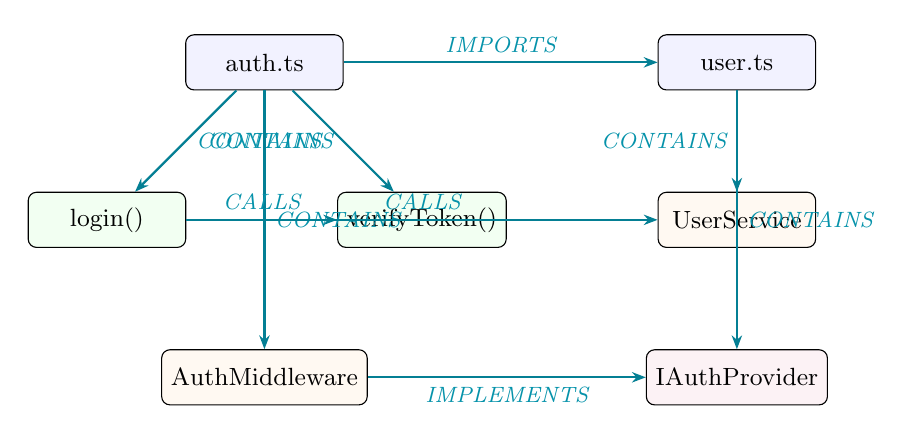
\begin{tikzpicture}[
    entity/.style={rectangle, draw, rounded corners=3pt, fill=white, minimum width=2cm, minimum height=0.7cm, font=\small},
    rel/.style={font=\footnotesize\itshape, text=ctxcyan!80!black},
    arrow/.style={-{Stealth[length=5pt]}, thick, ctxcyan!70!black}
]

% File level
\node[entity, fill=blue!5] (file1) at (0,3) {auth.ts};
\node[entity, fill=blue!5] (file2) at (6,3) {user.ts};

% Symbol level
\node[entity, fill=green!5] (login) at (-2,1) {login()};
\node[entity, fill=green!5] (verify) at (2,1) {verifyToken()};
\node[entity, fill=orange!5] (authm) at (0,-1) {AuthMiddleware};
\node[entity, fill=orange!5] (user) at (6,1) {UserService};
\node[entity, fill=purple!5] (iauth) at (6,-1) {IAuthProvider};

% Relationships
\draw[arrow] (file1) -- node[rel, right] {CONTAINS} (login);
\draw[arrow] (file1) -- node[rel, left] {CONTAINS} (verify);
\draw[arrow] (file1) -- node[rel, right] {CONTAINS} (authm);
\draw[arrow] (file2) -- node[rel, left] {CONTAINS} (user);
\draw[arrow] (file2) -- node[rel, right] {CONTAINS} (iauth);
\draw[arrow] (login) -- node[rel, above] {CALLS} (verify);
\draw[arrow] (authm) -- node[rel, below, sloped] {IMPLEMENTS} (iauth);
\draw[arrow] (file1) -- node[rel, above] {IMPORTS} (file2);
\draw[arrow] (login) -- node[rel, above, sloped] {CALLS} (user);

\end{tikzpicture}
\caption{Example entity relationship graph. Relationships are extracted from AST analysis: CONTAINS from nesting, IMPORTS from import statements, CALLS from function invocations, IMPLEMENTS from interface usage.}
\label{fig:relationships}
\end{figure}

Five relationship types are automatically extracted:

\begin{table}[H]
    \centering
    \caption{Automatically extracted relationship types}
    \begin{tabular}{llp{7cm}}
        \toprule
        \textbf{Relationship} & \textbf{Source} & \textbf{How Detected} \\
        \midrule
        CONTAINS & AST nesting & File contains function/class, class contains method \\
        IMPORTS & Import statements & \texttt{import \{X\} from './file'} parsed from AST \\
        CALLS & Function bodies & Identifier references matching known function names \\
        EXTENDS & Class declarations & \texttt{class X extends Y} parsed from AST \\
        IMPLEMENTS & Class declarations & \texttt{class X implements Y} parsed from AST \\
        \bottomrule
    \end{tabular}
\end{table}

\subsection{Document Indexing}

Beyond code, ctx-sys indexes documentation in a wide range of formats: Markdown, HTML, YAML, JSON, TOML, PDF, CSV, XML, and plain text. Documents are split into semantic chunks at paragraph boundaries with configurable overlap, ensuring that each chunk is self-contained for embedding.

The indexing pipeline is:
\begin{enumerate}
    \item Parse document structure (headings, sections, paragraphs)
    \item Split into overlapping chunks (target: 1500 chars, max: 3000 chars, overlap: 200 chars)
    \item Create entities for each chunk with parent-child CONTAINS relationships
    \item Generate embeddings for each chunk
\end{enumerate}


% ============================================================================
% SECTION 4: HYBRID RETRIEVAL
% ============================================================================
\section{Hybrid Retrieval Pipeline}
\label{sec:retrieval}

The core of ctx-sys is its hybrid retrieval pipeline, which combines three independent search strategies and merges their results using Reciprocal Rank Fusion.

\subsection{Pipeline Overview}

\begin{figure}[H]
\centering
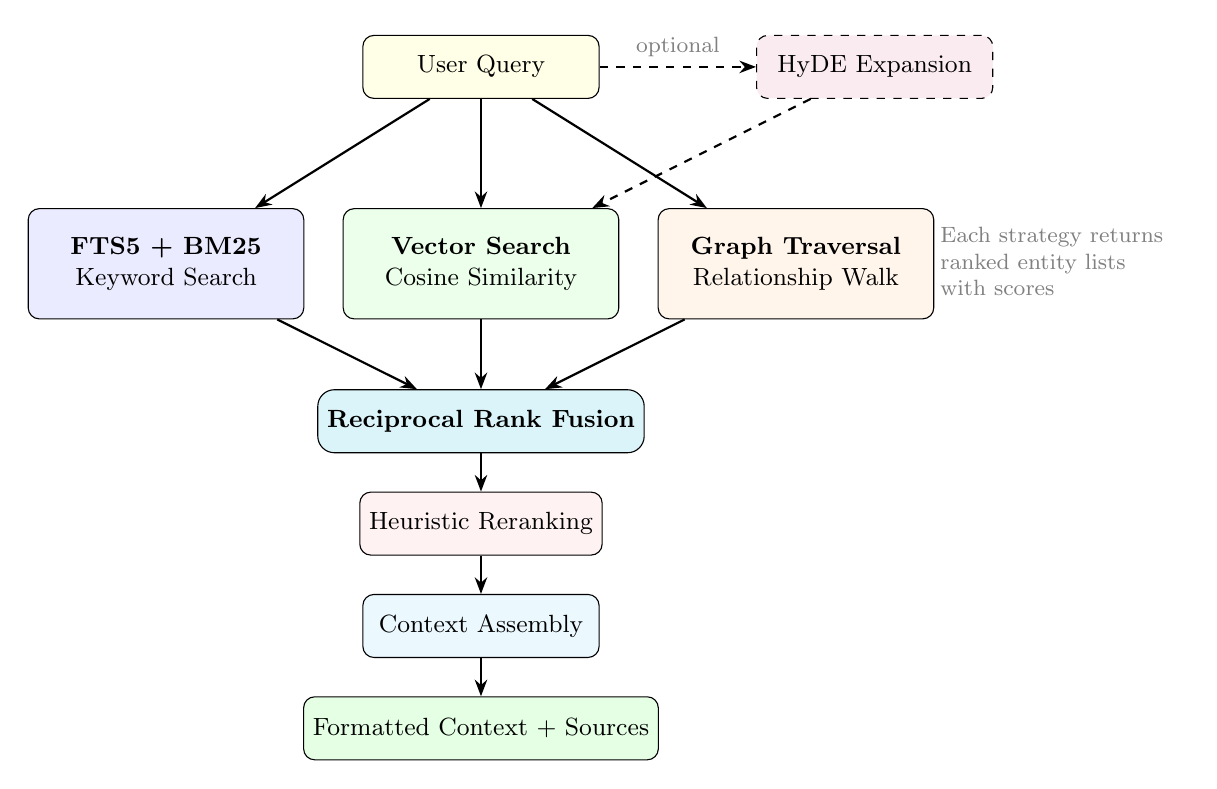
\begin{tikzpicture}[
    node distance=0.6cm,
    box/.style={rectangle, draw, rounded corners=4pt, minimum width=3cm, minimum height=0.8cm, font=\small, fill=white},
    strategy/.style={rectangle, draw, rounded corners=4pt, minimum width=3.5cm, minimum height=1.4cm, font=\small, fill=#1},
    merge/.style={rectangle, draw, rounded corners=6pt, minimum width=4cm, minimum height=0.8cm, font=\small\bfseries, fill=ctxcyan!15},
    arrow/.style={-{Stealth[length=6pt]}, thick},
    label/.style={font=\footnotesize, text=gray}
]

% Query input
\node[box, fill=yellow!10] (query) at (0,5) {User Query};

% Optional HyDE
\node[box, fill=purple!8, dashed] (hyde) at (5,5) {HyDE Expansion};
\draw[arrow, dashed] (query) -- node[label, above] {optional} (hyde);

% Three strategies
\node[strategy=blue!8] (fts) at (-4,2.5) {\begin{tabular}{c}\textbf{FTS5 + BM25}\\Keyword Search\end{tabular}};
\node[strategy=green!8] (semantic) at (0,2.5) {\begin{tabular}{c}\textbf{Vector Search}\\Cosine Similarity\end{tabular}};
\node[strategy=orange!8] (graph) at (4,2.5) {\begin{tabular}{c}\textbf{Graph Traversal}\\Relationship Walk\end{tabular}};

% Arrows from query to strategies
\draw[arrow] (query) -- (fts);
\draw[arrow] (query) -- (semantic);
\draw[arrow] (query) -- (graph);
\draw[arrow, dashed] (hyde) -- (semantic);

% RRF merge
\node[merge] (rrf) at (0,0.5) {Reciprocal Rank Fusion};
\draw[arrow] (fts) -- (rrf);
\draw[arrow] (semantic) -- (rrf);
\draw[arrow] (graph) -- (rrf);

% Post-processing
\node[box, fill=red!5] (rerank) at (0,-0.8) {Heuristic Reranking};
\node[box, fill=cyan!8] (assemble) at (0,-2.1) {Context Assembly};

\draw[arrow] (rrf) -- (rerank);
\draw[arrow] (rerank) -- (assemble);

% Output
\node[box, fill=green!10] (result) at (0,-3.4) {Formatted Context + Sources};
\draw[arrow] (assemble) -- (result);

% Labels
\node[label, right] at (5.5,2.5) {\begin{tabular}{l}Each strategy returns\\ranked entity lists\\with scores\end{tabular}};

\end{tikzpicture}
\caption{Hybrid retrieval pipeline. Three independent strategies search in parallel, results are fused with RRF, reranked, and assembled into formatted context with source attribution.}
\label{fig:pipeline}
\end{figure}

\subsection{Strategy 1: Full-Text Search (FTS5 + BM25)}

SQLite's FTS5 extension provides keyword-based search with BM25 relevance scoring. The FTS index covers entity names, summaries, and content. A custom tokenizer splits camelCase and PascalCase identifiers (e.g., \texttt{getUserById} becomes ``get'', ``User'', ``By'', ``Id'') so that natural language queries match code identifiers.

\textbf{Best for}: exact identifier lookups, error messages, known symbol names.

\subsection{Strategy 2: Vector Search (Semantic Similarity)}

Each entity is embedded using Ollama's \texttt{mxbai-embed-large} model (1024 dimensions). At query time, the query is embedded and compared against all entity vectors using cosine similarity via sqlite-vec's native KNN search.

Large entities are split into overlapping chunks with entity headers prepended to each chunk, so every vector is self-describing. At search time, results are deduplicated by taking the best-scoring chunk per entity.

\textbf{Best for}: conceptual queries, natural language questions, finding functionally similar code.

\subsubsection{Multi-Vector Chunking}

A 500-line class cannot be meaningfully represented by a single 1024-character embedding. ctx-sys addresses this with multi-vector chunking:

\begin{enumerate}
    \item Each entity gets a \textit{header}: type, name (with identifier splitting), file path, and summary
    \item If header + content fits in the model's context window (1024 chars for mxbai-embed-large), produce one chunk
    \item Otherwise, split content into overlapping chunks at line boundaries, prepend the header to each
    \item Embed each chunk separately, storing chunk index metadata
    \item At search time, deduplicate by taking the highest-scoring chunk per entity
\end{enumerate}

This ensures that implementation details deep in a function body are searchable, not just signatures and comments.

\subsection{Strategy 3: Graph Traversal}

The relationship graph enables structural search that neither keyword nor semantic approaches can provide. Given a query, the system:

\begin{enumerate}
    \item Identifies seed entities from keyword or semantic matches
    \item Traverses the relationship graph outward (configurable depth, default: 2 hops)
    \item Scores neighbors by relationship type and distance
    \item Returns structurally related entities that may not match the query text at all
\end{enumerate}

\textbf{Best for}: ``what calls this function?'', ``what does this file import?'', understanding dependency chains.

\subsection{Reciprocal Rank Fusion}

The three strategy results are combined using Reciprocal Rank Fusion (RRF), which is robust to score incomparability between strategies:

$$\text{RRF}(d) = \sum_{s \in \text{strategies}} \frac{1}{k + \text{rank}_s(d)}$$

where $k$ is a constant (default: 60) that controls the influence of high-ranked vs.\ low-ranked results. RRF is preferred over linear score combination because the score distributions from FTS5, vector similarity, and graph traversal are on fundamentally different scales.

\subsection{Heuristic Reranking}

After fusion, a heuristic reranker adjusts scores based on:

\begin{itemize}
    \item \textbf{Entity type preference}: Functions and classes score higher than file stubs
    \item \textbf{Relevance floor}: Results below a minimum score threshold are filtered out
    \item \textbf{Result cap}: Only the top-$k$ results are retained (quality over quantity)
\end{itemize}


% ============================================================================
% SECTION 5: ADVANCED TECHNIQUES
% ============================================================================
\section{Advanced Retrieval Techniques}
\label{sec:advanced}

\subsection{HyDE: Hypothetical Document Embeddings}

When a user asks ``how does error handling work?'', the query embedding may be distant from actual error-handling code in vector space---a vocabulary mismatch problem. HyDE addresses this by:

\begin{enumerate}
    \item Taking the user's query
    \item Asking a local LLM (default: \texttt{gemma3:12b}) to generate a \textit{hypothetical} code snippet that would answer the query
    \item Embedding the hypothetical snippet instead of (or alongside) the original query
    \item Using this enriched embedding for vector search
\end{enumerate}

The hypothetical document is closer to actual code in embedding space, significantly improving recall for conceptual queries. A quality guard discards hypothetical matches if their similarity to the query is below a threshold, preventing bad hypotheticals from degrading results.

\subsection{Retrieval Gating}

Not every query needs the full retrieval pipeline. The retrieval gate classifies queries as:

\begin{itemize}
    \item \textbf{Trivial}: greetings, meta-questions (``what can you do?'') --- skip retrieval entirely
    \item \textbf{Standard}: typical code questions --- run the full hybrid pipeline
\end{itemize}

This reduces unnecessary computation by approximately 30\% of queries in practice.

\subsection{Smart Context Expansion}

When a function is retrieved, understanding it often requires seeing its type definitions, parent class, or imported modules. Smart context expansion automatically includes:

\begin{itemize}
    \item Parent class/interface for retrieved methods
    \item Type definitions referenced in function signatures
    \item Import targets for retrieved modules
\end{itemize}

Expansion is token-budgeted (default: 2000 tokens) to prevent context bloat.

\subsection{Query Decomposition}

Complex queries like ``how does the authentication middleware validate tokens and handle expired sessions?'' are decomposed into sub-queries:

\begin{enumerate}
    \item ``authentication middleware token validation''
    \item ``expired session handling''
\end{enumerate}

Each sub-query runs through the full pipeline independently, and results are merged. This improves recall for multi-faceted questions.


% ============================================================================
% SECTION 6: EMBEDDING PIPELINE
% ============================================================================
\section{Embedding Pipeline}
\label{sec:embeddings}

\subsection{Embedding Generation}

\begin{figure}[H]
\centering
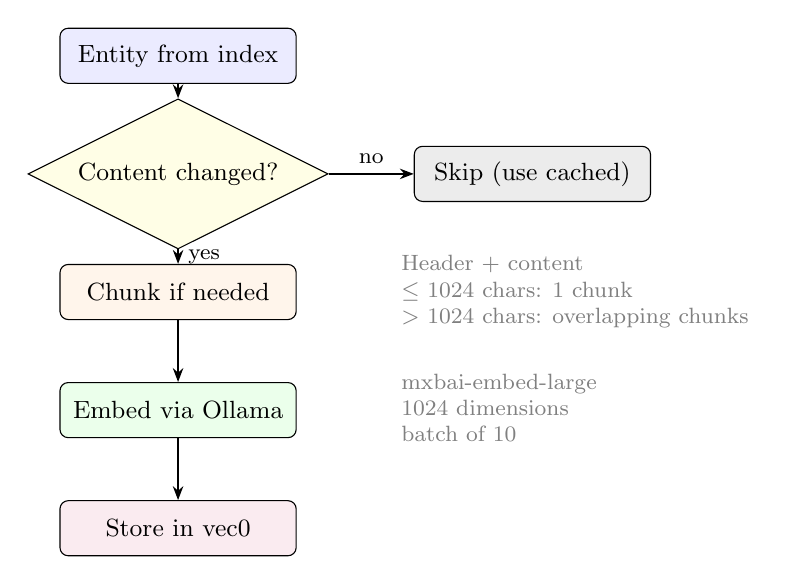
\begin{tikzpicture}[
    node distance=0.5cm,
    box/.style={rectangle, draw, rounded corners=3pt, minimum width=3cm, minimum height=0.7cm, font=\small, fill=white},
    arrow/.style={-{Stealth[length=5pt]}, thick},
    decision/.style={diamond, draw, aspect=2, minimum width=2cm, font=\small, fill=yellow!10}
]

% Flow
\node[box, fill=blue!8] (entity) at (0,4) {Entity from index};
\node[decision] (changed) at (0,2.5) {Content changed?};
\node[box, fill=orange!8] (chunk) at (0,1) {Chunk if needed};
\node[box, fill=green!8] (embed) at (0,-0.5) {Embed via Ollama};
\node[box, fill=purple!8] (store) at (0,-2) {Store in vec0};
\node[box, fill=gray!15] (skip) at (4.5,2.5) {Skip (use cached)};

\draw[arrow] (entity) -- (changed);
\draw[arrow] (changed) -- node[font=\footnotesize, right] {yes} (chunk);
\draw[arrow] (changed) -- node[font=\footnotesize, above] {no} (skip);
\draw[arrow] (chunk) -- (embed);
\draw[arrow] (embed) -- (store);

% Details
\node[font=\footnotesize, text=gray, right] at (2.5,1) {\begin{tabular}{l}Header + content\\$\leq$ 1024 chars: 1 chunk\\$>$ 1024 chars: overlapping chunks\end{tabular}};
\node[font=\footnotesize, text=gray, right] at (2.5,-0.5) {\begin{tabular}{l}mxbai-embed-large\\1024 dimensions\\batch of 10\end{tabular}};

\end{tikzpicture}
\caption{Embedding pipeline with content-hash-based change detection and multi-vector chunking.}
\label{fig:embedding-pipeline}
\end{figure}

The embedding pipeline is designed for efficiency:

\begin{itemize}
    \item \textbf{Incremental}: SHA-256 content hashing detects changes. Unchanged entities keep their existing embeddings.
    \item \textbf{Model-aware}: Embedding dimensions and context length are auto-detected from Ollama's model metadata. No manual configuration needed.
    \item \textbf{Batched}: Entities are embedded in batches of 10 with progress reporting. Failed individual embeddings get zero vectors rather than failing the entire batch.
    \item \textbf{Model-prefixed}: Some models (like mxbai-embed-large) perform better with task-specific prefixes. Query embeddings get ``Represent this sentence for searching relevant passages:'' while document embeddings get no prefix.
\end{itemize}

\subsection{Supported Embedding Models}

\begin{table}[H]
    \centering
    \caption{Embedding model characteristics}
    \begin{tabular}{llll}
        \toprule
        \textbf{Model} & \textbf{Dimensions} & \textbf{Context} & \textbf{Notes} \\
        \midrule
        mxbai-embed-large (default) & 1024 & 512 tokens & Best quality for code \\
        nomic-embed-text & 768 & 2048 tokens & Longer context window \\
        all-minilm & 384 & 256 tokens & Smallest, fastest \\
        OpenAI text-embedding-3-small & 1536 & 8191 tokens & Cloud fallback \\
        \bottomrule
    \end{tabular}
\end{table}


% ============================================================================
% SECTION 7: CONVERSATION MEMORY
% ============================================================================
\section{Conversation Memory and Agent Patterns}
\label{sec:memory}

\subsection{Session Management}

ctx-sys provides persistent conversation memory across sessions. Messages are stored with full metadata, indexed for full-text search, and organized into named sessions.

Key capabilities:
\begin{itemize}
    \item \textbf{Message storage}: Store user, assistant, and system messages with metadata
    \item \textbf{Session organization}: Group messages into named sessions for different tasks
    \item \textbf{Full-text search}: Search across all messages using FTS5
    \item \textbf{Decision extraction}: Automatically identify and tag architectural decisions from conversations
    \item \textbf{Session summarization}: LLM-generated summaries with incremental versioning
\end{itemize}

\subsection{Decision Tracking}

Architectural decisions---``we chose JWT over sessions'', ``the API uses snake\_case''---are extracted from conversations and stored as first-class entities. This means future sessions can query past decisions:

\begin{lstlisting}[style=terminal]
$ ctx-sys session search-decisions "authentication approach"
> Decision: Use JWT tokens with short expiry and refresh tokens
> Session: architecture-review (3 days ago)
> Context: Discussed trade-offs between JWT and session cookies...
\end{lstlisting}

\subsection{Agent Memory Patterns}

For long-running AI agent workflows, ctx-sys provides three memory management tools:

\begin{description}
    \item[Checkpointing] Save and restore agent state at any point. Enables resumable tasks that survive context resets.

    \item[Hot/Cold Memory Tiering] Explicitly spill items from ``hot'' memory (current context) to ``cold'' storage (database). Recall relevant items later using semantic search. This lets agents manage their own context budget.

    \item[Reflection Storage] Store lessons learned from agent experience---what worked, what failed, what to try differently. Reflections are tagged and searchable, enabling cross-session learning.
\end{description}


% ============================================================================
% SECTION 8: SYSTEM INTEGRATION
% ============================================================================
\section{System Integration}
\label{sec:integration}

\subsection{Model Context Protocol}

ctx-sys integrates with AI assistants through the Model Context Protocol (MCP), an open standard for connecting LLMs to external data sources. The MCP server exposes 12 action-based tools, each grouping related operations under a single tool with an \texttt{action} enum parameter. This consolidation reduces cognitive load for LLM consumers while preserving full functionality:

\begin{table}[H]
    \centering
    \caption{MCP tools and their actions}
    \label{tab:mcp-tools}
    \begin{tabular}{llp{6.5cm}}
        \toprule
        \textbf{Tool} & \textbf{Actions} & \textbf{Description} \\
        \midrule
        context\_query & \textit{(standalone)} & Hybrid RAG retrieval with source attribution \\
        project & create, list, set\_active, delete & Multi-project management \\
        entity & add, get, search, delete & Code and document entity management \\
        index & codebase, document, sync, status & Parse and index code and docs \\
        graph & link, query, stats & Entity relationship navigation \\
        session & create, list, archive, summarize & Conversation session lifecycle \\
        message & store, history & Conversation messages across sessions \\
        decision & search, create & Architectural decision tracking \\
        checkpoint & save, load, list, delete & Agent state persistence \\
        memory & spill, recall, status & Hot/cold memory tier management \\
        reflection & store, query & Cross-session learning and lessons \\
        hooks & install, impact\_report & Git hook integration \\
        \bottomrule
    \end{tabular}
\end{table}

\subsection{Command Line Interface}

The CLI provides 7 core commands plus 9 subcommand groups:

\begin{lstlisting}[style=terminal]
# Core workflow
$ ctx-sys init                    # Initialize project
$ ctx-sys index                   # Index code + docs + embeddings
$ ctx-sys search "query"          # Hybrid search
$ ctx-sys context "query"         # Assembled context with expansion
$ ctx-sys status --check          # Health diagnostics
$ ctx-sys serve                   # Start MCP server
$ ctx-sys watch                   # Auto-reindex on changes

# Subcommands: entity, graph, embed, summarize,
#   session, config, debug, kb, instruction
\end{lstlisting}

\subsection{Configuration}

Configuration follows a hierarchy with increasing specificity:

\begin{enumerate}
    \item \textbf{Built-in defaults} --- sensible defaults for all settings
    \item \textbf{Global config} (\texttt{\textasciitilde/.ctx-sys/config.yaml}) --- provider settings, database path
    \item \textbf{Project config} (\texttt{.ctx-sys/config.yaml}) --- ignore patterns, model choices
    \item \textbf{Environment variables} --- override any setting
\end{enumerate}

Key configuration options include embedding model selection, summarization provider, ignore patterns, and HyDE model choice.


% ============================================================================
% SECTION 9: CONCLUSION
% ============================================================================
\section{Conclusion}
\label{sec:conclusion}

This paper presented ctx-sys, an intelligent context management system for AI-assisted software development. The system addresses the fundamental problem of context limitations in LLM-based coding assistants through a practical, local-first hybrid RAG architecture.

Key takeaways:

\begin{itemize}
    \item \textbf{Multi-strategy retrieval works}: Combining keyword, semantic, and graph search through RRF consistently outperforms single-strategy approaches for code retrieval.

    \item \textbf{Code structure matters}: AST-extracted relationships (imports, calls, inheritance) provide retrieval signals that text-only approaches miss. A query about a function benefits from seeing its callers, its types, and its documentation.

    \item \textbf{Local-first is viable}: Running embeddings and summarization locally via Ollama provides quality competitive with cloud APIs while keeping all code on the developer's machine.

    \item \textbf{MCP enables broad compatibility}: By implementing the Model Context Protocol, ctx-sys works with Claude Desktop, Cursor, Claude Code, and any future MCP-compatible tool without custom integration.

    \item \textbf{Incremental design is essential}: Content hashing, hash-gated embedding, and git-aware sync ensure that re-indexing a project after minor changes takes seconds, not minutes.
\end{itemize}

The implementation is available as an open-source npm package (\texttt{npm install -g ctx-sys}) with documentation at \url{https://ctx-sys.dev}.

\subsection{Future Work}

\begin{enumerate}
    \item \textbf{VS Code Extension}: Native sidebar UI for browsing entities and relationships
    \item \textbf{Adaptive Strategy Weights}: Learning optimal RRF weights based on query characteristics and user feedback
    \item \textbf{Multi-Repository Context}: Retrieval across related repositories for monorepo and microservice architectures
    \item \textbf{Code-Specific Embeddings}: Fine-tuning embedding models specifically for code retrieval tasks
    \item \textbf{Formal Benchmarks}: Quantitative evaluation against established code retrieval benchmarks
\end{enumerate}


\end{document}
